\chapter{Implementation}
\label{cha:implementation}

This chapter of the Thesis looks at the implementation of the SMS algorithm for the modeling of vehicle noise for the LISTEN Project. Based on the theory discussed in Section \ref{cha:basic_principles}, this section looks at the details of the implementation, the changes and additions done the technique to improve it�s performance. Fine tuning, especially of the analysis part of SMS, was required to effectively and efficiently model the sound.

The implementation of the SMS algorithm, especially the analysis part, uses a number of constants which define the way the data is extracted from the recordings. These constants, or analysis parameters, have to be tuned for individual types of sounds depending on their interaction with the analysis.

%%%%%%%%%%%%%%%%%%%%%%%%%%%%%%%%%%%%%%%%%%%%%%%%%%%%%
\section{Source Data}
\label{sec:src_data}

The frequency contents of the source data, and other characteristics help to set up some analysis parameters required for the analysis of the sounds. Since the aim of this thesis project was to find good source models for vehicle sounds, a series was vehicle passage recording were used as source data to generate the models. The vehicles passing along a road were measured at a fixed point beside the road, hence recordings were said to be of a passage of the vehicle.

Table \ref{tab:vehicles} shows the vehicles used for the development and analysis of the SMS algorithm during this thesis project. The recordings were done largely in accordance with the measurement procedure of ISO 362-1:2007 \cite{ref:iso362}.

\begin{table}
\begin{center}
\begin{tabular}{ | l | l | l | }
    \hline
       Type & Brand & Model \\ \hline \hline
       Car & Opel & Astra \\
       Car & Volvo & V70\\
       Truck & Iveco & Daily (Medium Heavy) \\
       Bus & King Long & XMQ6127C \\ \hline
  \end{tabular}
  \caption{Types of vehicles used for source data.}
      \label{tab:vehicles}
   \end{center}
  \end{table}

The four type of vehicle at various speeds provide a variety sounds that can be used for source modeling. The Opel Astra was mainly used as for the comparison of results with another source modeling technique used previously. Having a range of source models allows the Auralization of a variety of specific scenarios, for example passage of a bus at regular intervals, or vary the rate and types of vehicles passing by simulating the amount of traffic throughout a day.

The source data was captured into PCM $.wav$ files, with a $44.1kHz$ sampling rate and $24bit$ resolution. The files were mostly unprocessed, except when certain occasions when unusual environmental conditions caused sounds not typical of a vehicle passage. For example a small stone on the road, which the vehicle rolled over, or birds chirping in the background could cause a unusual sound to be generated. Since the technique made a few assumptions on the source of sounds, based on the generation mechanism, it was not able to model such unusual sounds accurately. A few recording with such sounds were processed to filter out the unusual sounds.

%%%%%%%%%%%%%%%%%%%%%%%%%%%%%%%%%%%%%%%%%%%%%%%%%%%%%
\section{Peak Tracking}
\label{sec:peak_tracking}

Peak tracking is the most critical part of the Analysis stage. Peaks need to be accurately detected to model the tonal components. While theory discussed in Section \ref{sec:peakDet} provides a few methods of peak detection, many improvements can be done to the techniques to make them more effective and efficient.

The combination of a Discrete Fourier Transform (DFT), which is done during the Short Term Fourier Transform (STFT) and the source data, makes the spectrum very �peaky�. Hence, the detection algorithm finds multitudes of peaks. Some of these peaks in the spectrum are just noise which has a little more energy in a specific frequency component in that specific frame. While the DFT captures the frequency data in that specific frame accurately; considering over a few frames, the energy indicated by that specific peak could be categorized as noise. Thus, it is important to be able to differentiate between important peaks, which indicate presence of tones and less important peaks, which are just a part of the noise spectrum.

As discussed in Section \ref{sec:peakDet}, just the amplitude does not always indicate a the importance of a peak. A variety of other factors need to be considered including neighboring peaks and noise levels.

\subsubsection{Noise Threshold}
\label{sec:noise_threshold}

Quasi-stochastic noise is always modeled as having an average sound pressure level, often measured in dB with respect to maximum signal level allowed in the digitized signal. Depending on the timbre of the noise, this level changes over frequency. These noise levels are often considered as boundaries or thresholds. Any signal having amplitude below this threshold cannot be recovered separately from the noise. The auditory masking effect in human audio perception also makes such signals non-perceivable.

In the case of SMS Analysis, there are a couple of noise levels that can be considered and used at the peak tracking stage. Firstly, knowing an ambient and measurement noise level is effective in being able to differentiate between sounds (tonal or residual) which are a part of the recording and sounds which are external noise. A simple peak detection threshold that is set above this external noise level helps to avoid the detection of peaks caused by the ambient sounds. Such a threshold needs to be measured using the setup used for recording the real signal but with the noise source turned off. For the source material used in this thesis project, a recording made with the same equipment but without any vehicle passing by would yield such a threshold.

Furthermore, based on the assumption in the SMS technique of stochastic and tonal components of sounds, if the average level of stochastic noise of the source can be detected or calculated, that too can be used as a lower limit or threshold on the peak amplitude for detected peaks. Depending on source data measurement methods, sometimes it is possible to have data of vehicle passage with the engine turned off, which can be useful in estimating this noise threshold level. Since the engine noise is very tonal in nature, with that turned off, the noise of the tire-road interaction can be assumed to be quasi-stochastic in nature and hence the significant part of the residual component of SMS. Otherwise, a threshold can be set manually, based on inspection of the sound using a spectrogram looking at the level of the noise floor in comparison to maximum level corresponding to the maximum digital signal level. While, the actual noise floor is likely to be frequency dependent, the thresholds across all frequencies turns out to be a good estimate.

For the sounds used to implement and test the SMS technique, the levels used for noise thresholds are in Table \ref{tab:noiseTresholds}.

\begin{table}
\begin{center}
 \begin{tabular}{ | l | c | }
    \hline
       Noise & Treshold \\ \hline\hline
       Background (Ambient) & -70dB \\
       Noise Component & -55dB \\ \hline
  \end{tabular}
  \caption{Noise Thresholds used in the SMS Implementation.}
     \label{tab:noiseTresholds}
   \end{center}
  \end{table}


%%%%%%%%%%%%%%%%%%%%%%%%%%%%%%%%%%%%%%%%%%%%%%%%%%%%%

\subsubsection{Peak Width Thresholding}
\label{sec:peak_width_thresholding}

Mathematically, the width of a peak can be considered as the frequency bandwidth of the 3 dB drop in amplitude. This value is critical in being able to differentiate between a single, wide, peaks and multiple adjacent peaks. Section \ref{sec:peakDet} discusses peak shape with respect to the Fourier Transform of the window function used. Other factors affect the width of the peak as well. Interaction between multiple tones close in frequency can cause peaks to overlap, thus complicating the peak pattern.

The psyco-acoustical theory \cite{ref:psycho} also places importance on peak widths, in the light of the masking effect. A louder tone may mask off neighboring softer tones as masking effect makes tones of less amplitude within the same critical band non-perceivable. Such tones are redundant to be modeled, as they can't be heard by the listener. Hence, peaks too close to the other peaks can be ignored. Instead, detected peaks should be as far apart as possible from one another to avoid both the miss-detection of wide peaks, and redundant detection of masked tones.

The width of the peak can be calculated based on the window function, and used as a threshold to ensure no other peaks are detected within that range of a previously detected peak. However, the calculated peak widths tend to be a lot smaller than the frequency bandwidth in which tones can mask each other. Since, the threshold for the tones to be masked is not only a frequency bandwidth but also a difference in amplitude between the masker and the tones itself, a accurate pysco-acoustical masking model is complicated to implement and tune for peak detection.

A simpler hybrid solution is proposed in the implementing of the SMS technique for this project. The critical bands are defined by frequency intervals exponentially increasing in width with frequency. While the exponential increase of a full critical band bandwidth models the ears ability to distinguish individual tones very well, it is too large a segment of the frequency to consider for masking. This can be simplified by dividing each critical band into a number of sections. Each section can be allowed to have a single peak, which has the highest amplitude in that section. This ensures that peaks are far enough apart and don�t mask each other. Also wide peaks are not incorrectly detected as multiple peaks due to this method. Figure \ref{fig:CritBandSections} illustrates the critical bands and their sections on a logarithmic frequency scale.

\begin{figure}
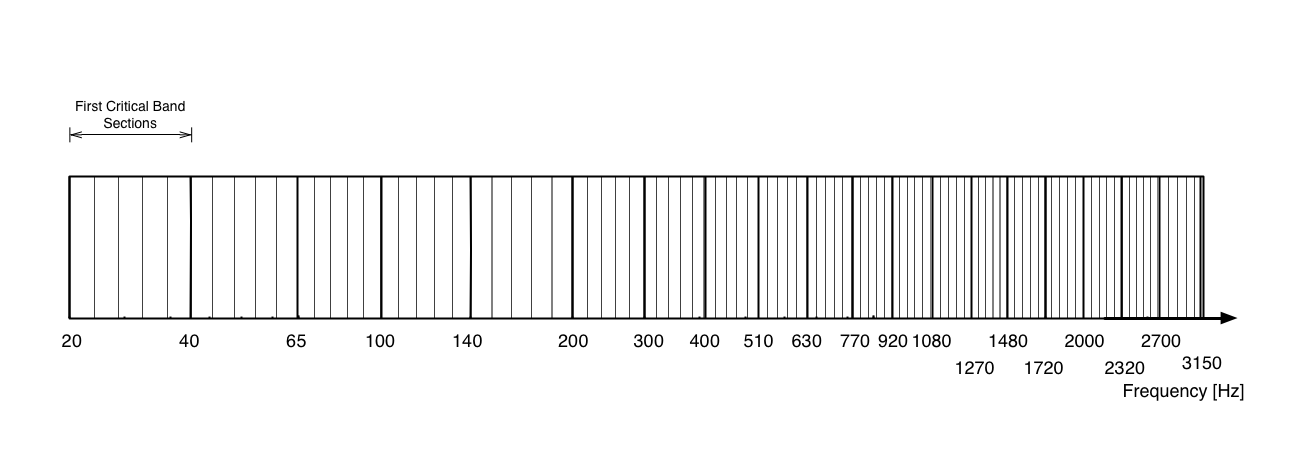
\includegraphics[height=5.5cm]{../images/CritBandSections.png}
\caption{Illustration of Sections in Critical Bands with 5 sections in each band for bands from 20 Hz till 3150 Hz in log scale.}
\label{fig:CritBandSections}
\end{figure}

The number of sections per critical band is a parameter which has to be manually tuned for the source data being used. A larger number would mean that the allowed peaks would be closer to each other and could detect some redundant peaks. A smaller number may not be able to track all the tones present in the sound. A number between 5 and 25 was seen to be appropriate in the case of the vehicle sounds. There are ways to automate the detection and tuning of this parameter that have not been explored in this thesis.

%%%%%%%%%%%%%%%%%%%%%%%%%%%%%%%%%%%%%%%%%%%%%%%%%%%%%

\subsubsection{Peak Amplitude Calculation}
\label{sec:peak_amp_cacl}

Two methods have been discussed in Section \ref{sec:peakDet} for the detection and calculation of Peak Amplitude. The quadratic interpolation based method proposed by Serra \cite{ref:sms} and the derivative signal based method proposed by Desainte \cite{ref:accuratePeak}.

While the division operation between the two magnitude spectra in derivative method cancels the effect of the analysis window on the peak amplitude and frequency; in the quadratic interpolation method, the peak amplitude is still affected by the window function.

A window function is used in the STFT analysis to enforce periodicity on the signal and avoid generation of nonexistent high frequency information. However, a window function reduces the energy in the signal as the signal amplitude is tapered down at the ends. In the transform domain, it can be considered as a convolution with the Fourier Transform of the window function with the spectrum of the signal. This is show in Eq. \ref{eqn:windowTransform},

\begin{eqnarray}
\label{eqn:windowTransform}
STFT\{x[n]\} \equiv  X[m,\omega] & = \sum_{n = -\infty}^{\infty}x[n]w[n-m]e^{-j\omega n}\\
& = X_m[n] \cdot W[n]
\end{eqnarray}

where, $x[n]$ is the signal being analyzed, $w[n]$ being the sliding window used, $X_m[n]$ is spectrum of the signal and $W[n]$ is the spectrum of the window.

Hence at the peak, the amplitude of the spectrum would be scaled by a factor that is given by the magnitude of the Fourier Transform of the window function at the center of the window. This is known as the coherent gain factor of the window. This factor corrects the amplitude of the peak. This is crucial as the amplitude of a tone in SMS is calculated using the peak amplitude.

The derivative signal based method proposed by Desainte however needs the continuous value of the Fourier Transform of the window function to be able to calculate the accurate peak amplitude. Since the Fourier Transform of the window functions is not always possible to calculate analytically, a high resolution discrete Fourier Transform is used instead. This simulates a continuous valued Fourier Transform, assuming a gradually changing spectrum. This is computationally slow and has to be 'cached' to improve the analysis computational performance.

Both techniques are implemented for the project and can be used interchangeably. A very little difference was seen in the values generated using the two techniques.

%%%%%%%%%%%%%%%%%%%%%%%%%%%%%%%%%%%%%%%%%%%%%%%%%%%%%
\subsubsection{Peak Ordering}
\label{sec:peak_orderings}

When the peaks are detected they have to be ordered in terms of their importance for the assignment to various trajectories. The ordering of the peaks can be done based on their amplitude, but as suggested by Serra, X. \cite{ref:sms} importance has to be given to the difference between the peak amplitude and the nearest valley amplitude. Tones with the greatest amplitude with respect to all other tones in that critical band are more perceptible \cite{ref:psycho}, and hence more important in modeling the sound.

A simpler implementation of this is based on ordering of the peaks. Instead of searching for the nearest valley, the gradient of each peak is considered as the metric to order the peaks by. The higher the gradient, the larger the difference between the peak and the nearest valley. The gradient in this case is defined as Eq. \ref{eqn:gradCalc}, where $x[n]$ is the signal and $n_p$ is the detected index of the peak. This assumes that the valley is always one index away from the peak, which is true in most cases with noisy signals as in the case of vehicle sounds with the STFT parameters used in this thesis project.

\begin{equation}
\label{eqn:gradCalc}
G_i = X[n_p]-X[n_p-1]
\end{equation}

%%%%%%%%%%%%%%%%%%%%%%%%%%%%%%%%%%%%%%%%%%%%%%%%%%%%%
\subsection{Frequency Guides}
\label{sec:freq_guides}

Frequency guides are virtual guides that track the peaks for each subsequent frame and form a trajectory of peaks defining amplitude and frequency of quasi-sinusoidal waveform. The generation, decay and advancement of the guides affect the shape of the trajectory and hence the final model. Guides allow gradual change of amplitude and frequency of the sinusoids, thus the parameters and the processes of the guide advancement are critical in being able to track the tonal components well.

Since the original source was a recording of a passage of vehicles, the Doppler effect causes a shift in frequency of the sound at the instance of passage. This shift also has to be detected and tracked accurately in the frequency guides.

%%%%%%%%%%%%%%%%%%%%%%%%%%%%%%%%%%%%%%%%%%%%%%%%%%%%%
\subsubsection{Guide State Machine}
\label{sec:guide_state_mac}

The virtual frequency guides are given states to allow guides to �sleep� as discussed in Section \ref{sec:peakTrack}.  A finite state machine implements the various states of the guides. This allows the state transitions to be defined, and the appropriate actions to be taken when the state transitions happen. Such a process of tracking the guides becomes more useful when further processing is done as the guide finds an appropriate peak while in the �sleep� or dormant state or as a guide needs to process the tracked tones and smoothen its trajectory.

Figure \ref{fig:fGuideStateMachine} shows a state diagram which defines the state machines of the frequency guides. Many state transitions are not allowed and only a few result in specific actions.

\begin{figure}
\begin{center}
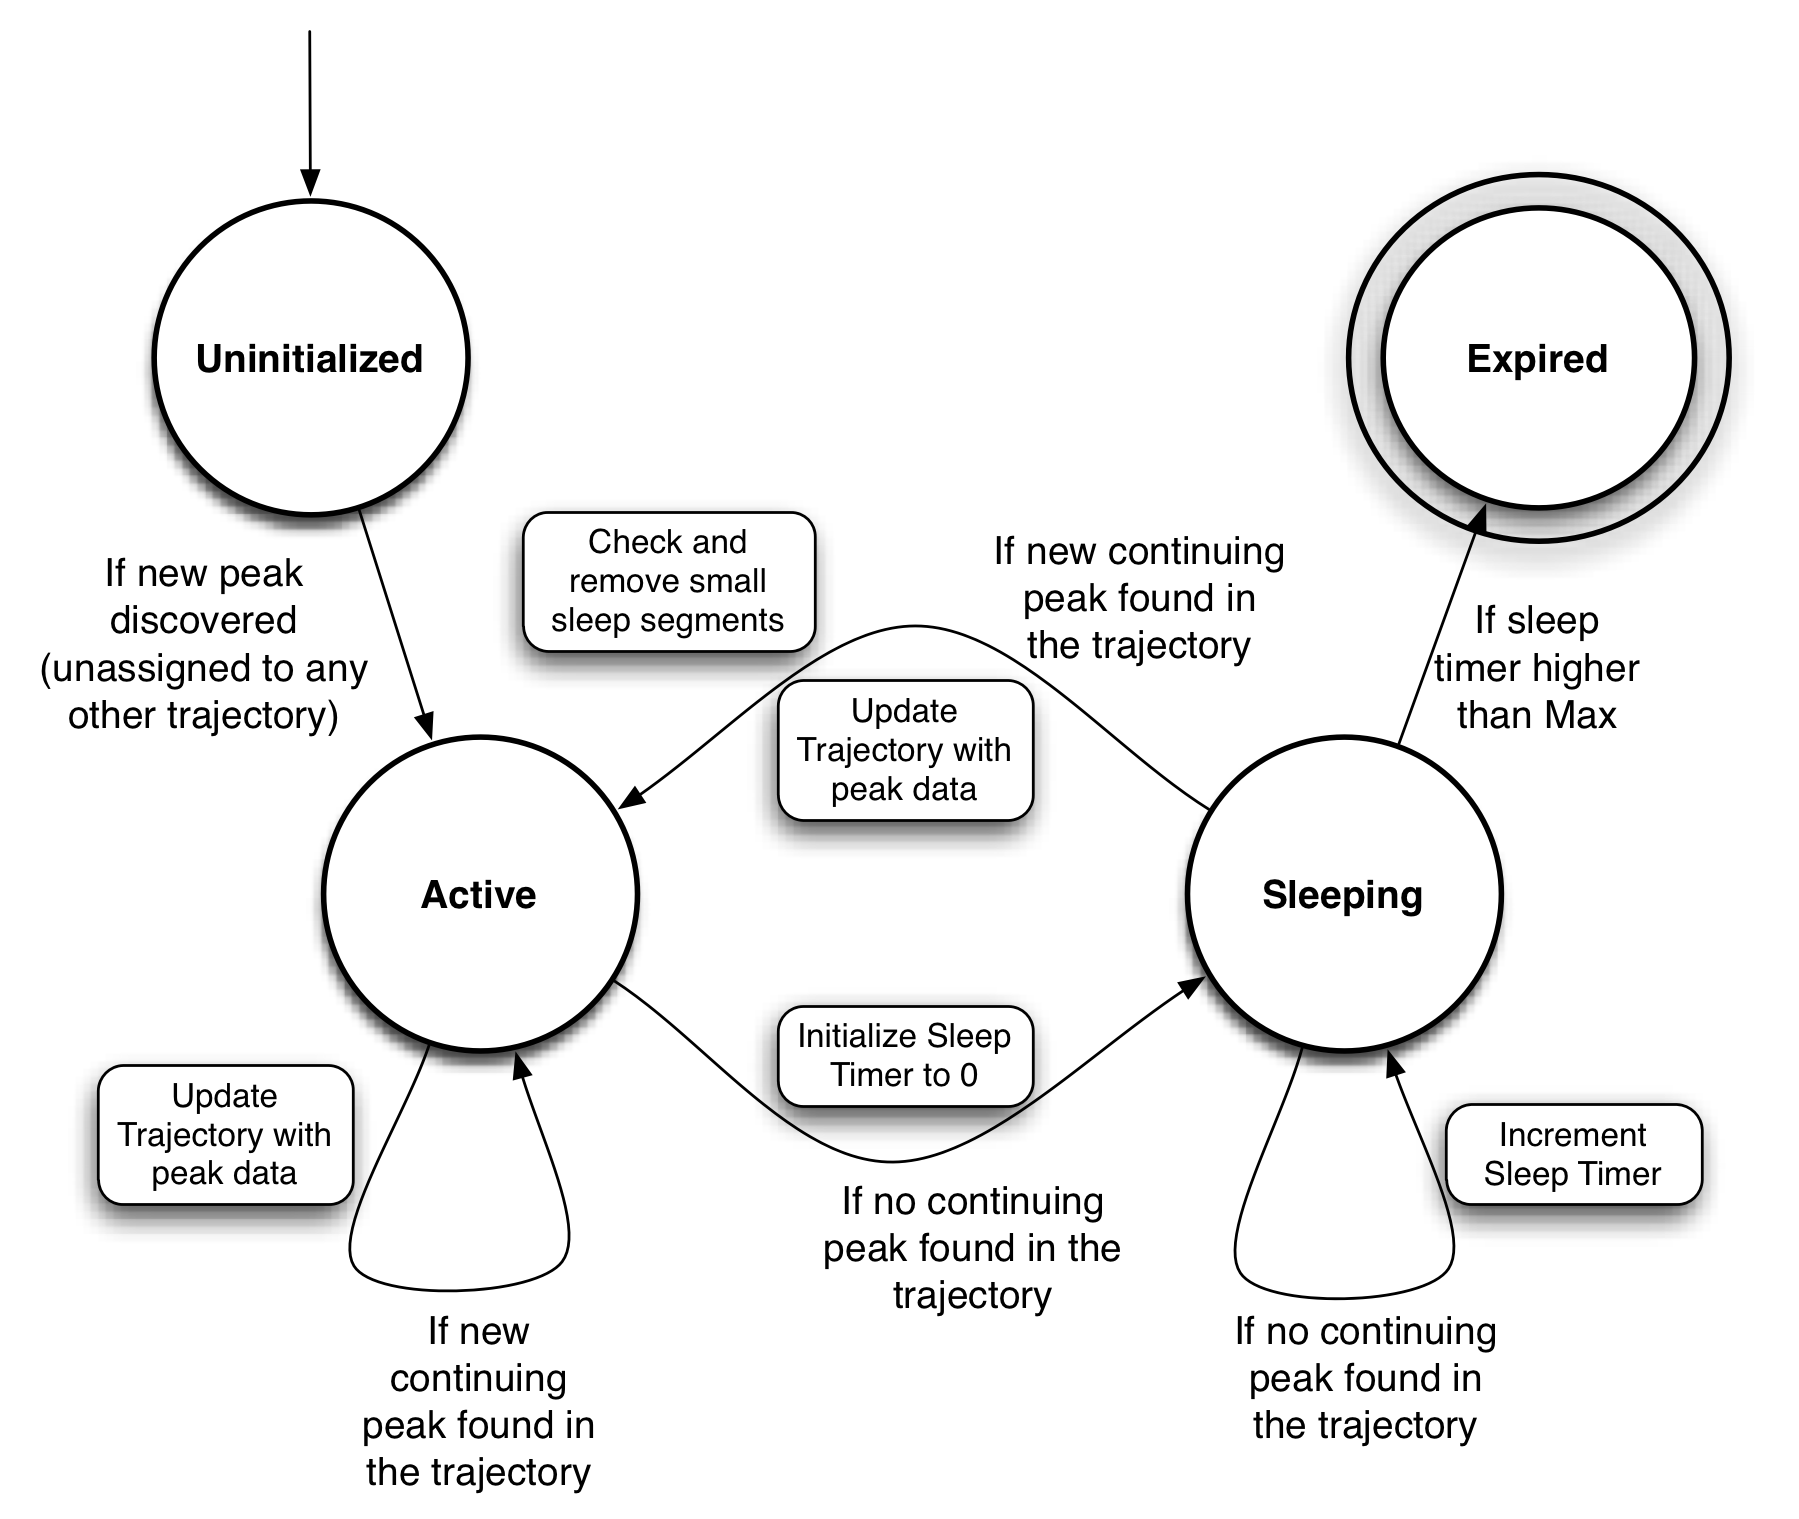
\includegraphics[height=9.0cm]{../images/FGuideStateMachine.png}
\label{fig:fGuideStateMachine}
\caption{Frequency Guide State Machine Diagram.}
\end{center}
\end{figure}


%%%%%%%%%%%%%%%%%%%%%%%%%%%%%%%%%%%%%%%%%%%%%%%%%%%%%
\subsection{Guide Width}
\label{sec:guide_width}

Similar to the peak width, the width of a frequency guide is a parameter which needs to be tuned depending on the sound. The width of the guide allows the guide to accept peaks within the range of the width around the center frequency of the guide. A wider guide accepts peaks of frequencies that are far from the current center frequency. This ensures that the guide does not �expire� quickly as a result of a lack of appropriate peaks. However, a wider guide tends to allow the trajectories to deviate significantly. This might cause confusion with if the sounds have two tonal components that are less than the guide width in frequency apart. In such a case, the frequency guide will tend to jump between the peaks from each of the component, yielding an unnatural sound.

The control of the guide width is critical in being able to detect correct trajectories. Once again the perceptual critical band theory can be used to ensure that the band-with is wide enough to detect differences between perceivably distinct tones, and yet not too narrow as to not allow the gradually changing tones, like a Doppler shift to be captured within a single guide.

Based on the critical band section method used in peak detection, a similar sections based simplification can be used to define guide widths. Each critical band can be divided into a number of sections; within each only a single frequency guide is allowed to exist. This ensures that the guides are far away from each other and do not deviate too much from the center frequency to track peaks, which may lead them to track peaks from another tone.

Once again, the number of sections per guide is a parameter that needs to be tuned to be able to extract tones accurately. Throughout the implementation of the SMS technique, values between 5 and 20 were used for the number of sections generated from critical bands. A higher number tended to offer better results in vehicle sounds as the tones in the source data did not vary much from the original frequency.

%%%%%%%%%%%%%%%%%%%%%%%%%%%%%%%%%%%%%%%%%%%%%%%%%%%%%
\subsection{Trajectory Frequency Smoothing}
\label{sec:guide_freq_smoothing}

Frequency Guides help to detect and shape a trajectory of peaks. To ensure a gradual change in the frequency of the sinusoid modeled by the peaks, the trajectory frequencies need to be smoothed. This is done as proposed by Serra using a current trajectory bias which is based on a simple low pass filter expression. The progression of the guide is based on a weighted sum of the current trajectory of the guide and the new peak being tracked, thus smoothly shifting towards the new peak.

Eq. \ref{eqn:guideFreqSmoothing} shows the expression used to calculate the influence of new peaks on the trajectory, where $\hat{f}_i$ is the estimate frequency of the next peak based on the current trajectory, and $g_i$ is the frequency of the next peak being tracked, and $f_i$ is the final frequency assigned to the guide after the smoothing.

\begin{equation}
\label{eqn:guideFreqSmoothing}
f_i = \alpha(g_i-\hat{f}_i) + \hat{f}_i
\end{equation}

The constant $\alpha$ is used to decide wether the current trajectory is given more importance or if the new peak�s frequency is given more importance when deciding the frequency of the trajectory for the next frame.

This parameter $\alpha$ allows the smoothness of the frequency guide to be adjusted. An $\alpha$ with a value close to 1 favors the frequency of the new peak, while an $\alpha$ with a value of 0 favors the extrapolation of the current trajectory. $\alpha$ is also a parameter which has to be tuned for accurate analysis of the model. Mostly in the implementation of the SMS Technique, an $\alpha$ value of between 0.25 and 0.4 was used. A moderate value of alpha allowed a smooth tracking of peaks and yet still track sudden large changes in frequency like seen during a Doppler shift at the point of passage.

%%%%%%%%%%%%%%%%%%%%%%%%%%%%%%%%%%%%%%%%%%%%%%%%%%%%%
\subsection{Trajectory Amplitude Interpolation}
\label{sec:guide_amp_interpolation}

Along with a smoothly changing frequency of the trajectory of the tone, the amplitude of the tonal component is also assumed to be smoothly changing. Hence, the trajectory amplitudes are interpolated to give a smoothly changing amplitude value for the sinusoids between individual peaks.

Although this interpolation yields a smooth change between subsequent frame, the amplitude of the peaks themselves can vary significantly and might change drastically if no peak is found in the current guide, forcing the guide to go into "Sleep" mode. The negative effect of this is having Frequency Guides that �sleep� and �awake� in rapid succession. The Auralization of such trajectories where peaks often have zero amplitude, have artifacts that sound unnatural. This behavior was seen often in signals with amplitudes that are close to the noise threshold.

To reduce these artifacts, a trajectory is analyzed at the end of the peak tracking operation and short sleep periods of Frequency Guides are removed and replaced with guessed values. The definition of short is again another parameter that needs to be tuned. However, the value of this period may be calculated, based on the time interval needed to perceive the decay of a tone, and thus it would depend on the hop length. Eq. \ref{eqn:peakLowerLimit} shows the expression which could be used for this,

\begin{equation}
\label{eqn:peakLowerLimit}
N_{limit} = \lfloor \frac{T_{min}\times f_s}{M}\rfloor
\end{equation}

where $M$ is the hop length, $T_{min}$ is the minimum time for a sleep period not to be interpolated, and $f_s$ is the sampling frequency.

Care needs to be taken though as interpolating over a larger time period may add energy to the tonal component that might not exist in the original sound causing inaccuracies in the model.

The removal of the sleep period can be implemented by setting the peak amplitude for the frames during the sleep period to values based on simple linear interpolation between amplitudes of the last peak before the Frequency Guide went into sleep state and the first peak after it comes out of sleep state. These allows the tone to change gradually between the two states and not auralize artifacts caused by rapidly changing amplitudes.

For the SMS Implementation a nominal value of 0.5 seconds was considered as the minimum sleep duration, and any sleep period less than that was removed using the interpolation described above. Eq .\ref{eqn:ampInterpolation} gives the formula used for the interpolation,

\begin{equation}
\label{eqn:ampInterpolation}
A^{\prime}_i = \frac{(A_{first}-A_{last})}{(first-last)}\times i + A_i
\end{equation}

where $A_i$ is the original peak amplitudes before interpolation, $A_{first}$ is the amplitude of the first peak after the sleep mode, and $A_{last}$ is the amplitude of the last peak before sleep mode.

%%%%%%%%%%%%%%%%%%%%%%%%%%%%%%%%%%%%%%%%%%%%%%%%%%%%%
\subsection{Guide Energy Filtering}
\label{sec:guide_energy_filt}

Noise thresholding as defined in Section \ref{sec:noise_threshold} helps to reduce the number of redundant peaks. A smaller number of peaks allows a quicker tracking and Auralization of peaks. However that has to be balanced with having very little or no perceptual change the sound. It was observed during testing that sometimes lesser peak trajectories yielded sounds perceptually more similar to the original than if more trajectories were used, as many of the extra peaks tracked and auralized were not from the tonal component but noise peaks which were mistakenly tracked as tones.

Thus, it is useful to remove trajectories that do not contribute much to the final sound from the rest of the analysis. This can be done by a simple energy comparison. A value representing the energy of each peak trajectory can be calculated using the Eq. \ref{eqn:energyFilt},

\begin{equation}
\label{eqn:energyFilt}
E_j = \sum_i A_{i,j}^2\times M_j
\end{equation}

where, $A_{i,j}$ is the i-th peak in the j-th Frequency Guide, and $M_j$ is the hop length of the the j-th guide.

While the value may not reflect the exact amount of energy in the sound synthesized by the trajectory, it is the relative value between the trajectories which can be compared to decide which trajectories can be ignored.

A simple percentage of energy comparison can help in the detection of redundant guides. Any trajectories with total energy less than a specific percentage of the combined energy in all the guides, can be ignored.  This is another parameter that has to be tuned to ensure that the appropriate number of trajectories should be considered. During the experiments, a value between 0.1\% to 0.05\% seemed to be appropriate.

%%%%%%%%%%%%%%%%%%%%%%%%%%%%%%%%%%%%%%%%%%%%%%%%%%%%%
\subsection{Guide limit increments}
\label{sec:guide_limit_inc}

Even with noise tresholding, there are many peaks that get detected which do not correspond to a specific tonal component. However, since that cannot be verified until no other peaks are found in the subsequent frames, all new peaks get assigned a new frequency guide. This generates a large number of guides, which might not continue beyond a few frames, and hence the total number of guides keeps increasing every frame analyzed. This can quickly get computationally challenging. Hence, a simple limit on the maximum number of guides ensures that only the important peaks can generate new trajectories. And since the peaks are assigned to guides in the order of their amplitudes (or gradient as described in Section \ref{sec:peak_orderings}) only the important peaks are assigned before the limit of number of guides is reached.

With a limit on the maximum number of guides, the limit gets reached very quickly within the first few frames. Hence, if an actual tonal component starts midway through the sound, there might not be any frequency guides left to track it. This is not a common effect in musical sounds, where the tonal components are more or less stationary and begin from the start of the sound. But in environmental sounds it is common to have tones that become significant much later in the sound as a result of propagation or other effects.

A proposed solution is to allow additional guides to be added to the tracking algorithm as the further frames are tracked. Eq. \ref{eqn:guideInc} shows the change of the maximum guide limit can have with more and more frames are added,

\begin{equation}
\label{eqn:guideInc}
N_{g,i} = \frac{4\times N_{g,init}\times c_{inc}\times i}{3\times N_{hops}} + N_{g,init} \hspace{20pt} \forall i \in [1, \frac{3 \times N_{hops}}{4}]
\end{equation}

where, $N_{g,init}$ is the limit of the number of frequency guides at the beginning of the peak tracking process, $N_{hops}$ is the total number of hops, $c_{inc}$ is the increment factor, which is the fraction of the $N_{g,init}$ which are added through the tracking process.

This increase of the limit can be stopped nearer to the end as not many new tones start close to the end of the sound. Experiments show that a guide limit increase for the first 75\% of all the frames is enough to deal with most late starting tonal components.

Here, the guide limit, or the maximum number of guides allowed is an analysis parameter that needs to be tuned. The tuning of this parameter is a direct trade-off between the quality of model and the amount of computational time required to synthesize the sounds. Similarly, the increment factor is also a parameter that needs to be tuned for the specific sound being analyzed. Complex sounds with new tones starting at various instances through out the sound might need a higher increment factor.

%%%%%%%%%%%%%%%%%%%%%%%%%%%%%%%%%%%%%%%%%%%%%%%%%%%%%
\section{Noise Synthesis}
\label{sec:noise_synth}

A number of implementation improvements also need to be done in the Noise Synthesis part of the SMS method. During the Noise synthesis operation, the residual spectrum is first interpolated from the parameters and then assigned random phase before being transformed to the time domain by an Inverse Fourier Transform.

\subsection{Phase Randomization}
\label{sec:phase_rand}

Randomization of the phase assigned to the spectrum serves two purposes. Firstly, the frequency domain subtraction method used to calculate the residual, does not generate the phase of the residual spectrum. Hence, there is a need to generate the phase for the spectrum. Furthermore, since the specific phase information is not perceivable in a noise component, it does not need to be stored and can be generated randomly. Serra suggests using a uniform random variable with values between $0$ and $2\pi$ or $-\pi$ and $\pi$ to generate the phase.

However, to generate a real signal from the complex spectrum using the Inverse Discrete Fourier Transform (IDFT), the spectrum has to have a certain format. The complex spectrum of a real signal is always mirrored and conjugated. Thus the random phase can be assigned to the half of the magnitude spectrum that has been interpolated, and the resulting complex spectrum can be mirrored and concatenated to make the complete complex spectrum. Eq. \ref{eqn:randPhaseSt} - \ref{eqn:randPhaseEd} explains this operation.

\begin{eqnarray}
\label{eqn:randPhaseSt}
\theta_l(n) = & 2\pi\times rand(\frac{N}{2}-1) \\
\theta_r(n) = & -\theta_l(\frac{N}{2}-1 -n)\\
\theta = & [0, \theta_l(n), 0, \theta_r(n)]
\label{eqn:randPhaseEd}
\end{eqnarray}

Here, $rand$ is a random number generator which produces a vector of random numbers between $0$ and $1$. Scaling it to $2\pi$ gives a vector of random numbers between $0$ and $2\pi$. The phase vector needs a value of 0 at the 1st index and at the N/2+1st index. The random vector, $\theta_l$ is then mirrored, conjugated and concatenated to give the final phase vector, $\theta$. The IDFT can be calculated from the phase vector and the magnitude using Eq. \ref{eqn:resSynthSpec}.

\subsection{Overlap and Add of Synthesis}

The zero padding used in the DFT/IDFT operation for residual synthesis breaks the duality of Sliding Window analysis and Overlap and Add synthesis. Zero padding is used in DFT operations to improve the accuracy of the spectrum by decreasing the difference in subsequent discrete frequencies in the spectrum. Generally, at least twice the length of the analysis window length is recommended as the length of the padded signal.

However, this creates a spectrum of the same length at the padded signal. Without any other process, if this spectrum is transformed back into time domain waveform using IDFT, it will contain the original windowed signal concatenated with the zero padding. However, during the residual synthesis, the phase of the complex spectrum is randomized. The re-transformed time-domain signal does therefore not have any identifiable zeros padding concatenated at the end of the waveform, and is still of the same length as the padded waveform. Figure \ref{fig:zeroPaddingIDFT} illustrates this for an arbitrary signal. The inverse Fourier transform of the spectrum without any changes yields the original time domain signal with the identifiable zero padding at the end (bottom-left plot). However the same magnitude spectrum when combined with a random phase and inverse Fourier transformed does not give a time domain signal with a clear zero padding (bottom-right plot).

\begin{figure}[ht]
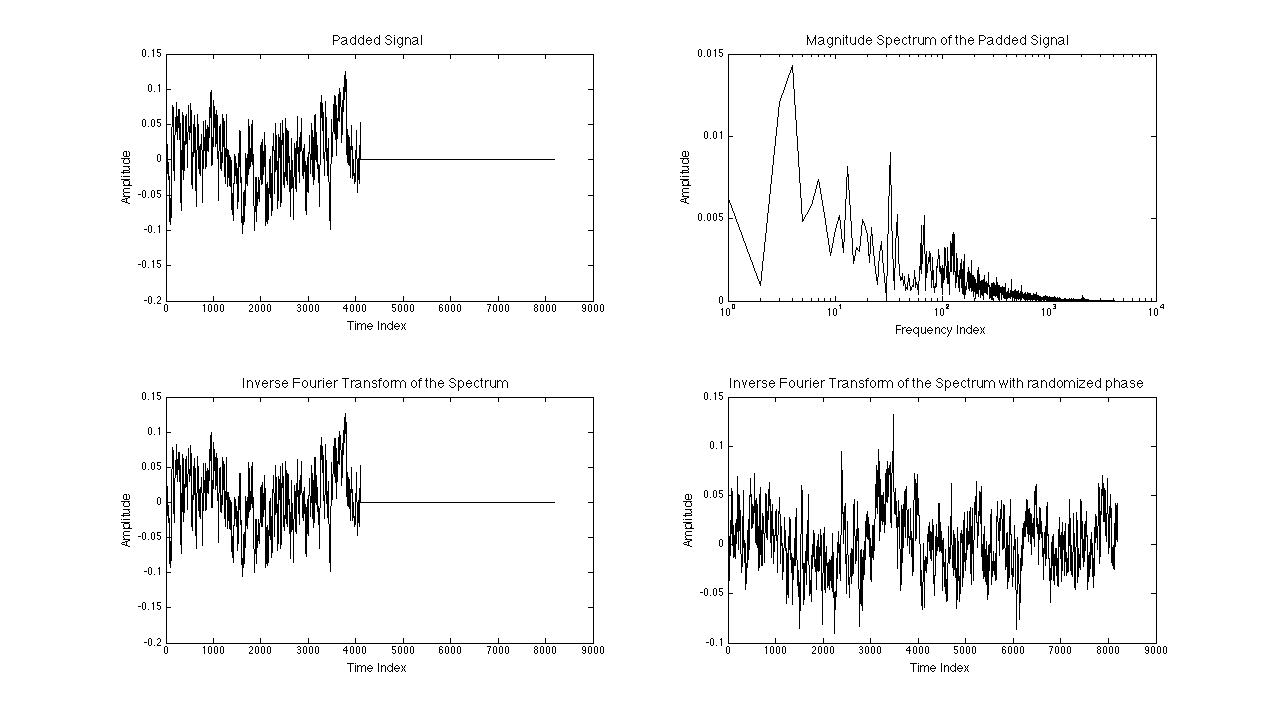
\includegraphics[height=9.0cm]{../images/IDFTPadding.png}
\caption{Example plots of (clock wise from top left) an Original Signal, its Magnitude Spectrum, and the Inverse Fourier Transform of the Magnitude Spectrum with and without randomized phase information.}
\label{fig:zeroPaddingIDFT}
\end{figure}

While total energy is still the same, and also at the same frequency (since the spectrum is similar), it is now spread out over the entire signal instead of being concentrated in the initial part of the signal. In other words, since the phase of each of the frequency content in the original signal was discarded and replaced with random phase, the energy in the various frequencies shifted in the time domain.

Since now the signal is longer, it cannot be overlapped and added the same way as the original signal with the zero padding which could be identified and removed before the overlapping. To overcome this, the signal has to be truncated to the length of the analysis window. This truncation of data can cause the loss of information in some frequencies. However, the nature of zero padding does not add any information to the signal and hence all the relevant frequency information can be proven to be captured within the part of the signal which remains after truncation.

Furthermore, since the net energy was spread out over the entire signal, some of it is lost in truncation here, as the truncated part of the signal is not non-zero unlike the case with zero padding. Thus, the signal left after the truncation has to be scaled to have the same amount of energy as original in order to have similar loudness. Here too, the redundancy of the actual noise distribution helps to ensure that the perception of the type noise is not altered. The scaling can be expressed as defined in Eq. \ref{eqn:zeroPadTrunc},

\begin{eqnarray}
x^\prime_r = x_r[1:N_o]\times \frac{N_z}{N_o}
\label{eqn:zeroPadTrunc}
\end{eqnarray}

where $N_o$ is the original window length, $N_z$ is the window length with the zero-padding, and $x_r$ is the time domain signal of a specific frame after synthesis.

After the truncation and scaling, with a residual synthesis waveform of each frame being the same length as the original waveform, overlap and add synthesis will give an perceptually accurate reconstruction of original signal.

\subsection{Weighted Overlap and Add}
While the COLA constraint (see Section \ref{sec:COLA}) ensures that a Sliding window based STFT and an Overlap and Add process keeps the original signal constant, it does not take into account the processing of the signal between the two. The process of parameterizing the noise envelope (as defined in Section \ref{sec:residualparam}) affects the noise signal itself. When the residual is originally calculated, the STFT of the original and the re-synthesized tones are used. Since the STFT process windows the signal before they're subtracted, each residual/noise Hop can be considered to be windowed. Eq. \ref{eqn:windowednoise} shows the analog of the frequency domain subtraction in time domain:

\begin{eqnarray}
\label{eqn:windowednoise}
r_m[n] = x_m[n] - x_{r,m}[n]
r_m[n] = x[n]w[n-mR] - x_r[n]w[n-mR]
r_m[n] = w[n-mR](x[n] - x_r[n])
\end{eqnarray}

Here, $x_m$, $x_{r,m}$, $r_m$ are the original, re-synthesized tone and residual signal respectively, of the $m$th Hop.

The process of parameterization, interpolation as well as synthesis using the random phases (see Section \ref{sec:residualcalc}) causes the re-synthesized residual signal to loose it's windowed amplitude. Hence, in order for the overlap and add to work, it needs to be windowed again. Thus the finally re-synthesized noise signal has gone through windowing twice. Hence the COLA constraint cannot be applied to it directly. Instead a weighted version of the COLA constraint, Weighted Overlap and Add (WOLA) as defined by Smith \cite{ref:smith} can be used.

Since the residual signal is windowed twice during the entire SMS process, it has to be constant after the overlap and add process when the square of the window function (same window applied twice) is applied to it. Smith recommends using the same window both the times for ease of finding a WOLA constant combination of window and overlap ratio. Eq. \ref{eqn:wolaEqn} defines the new WOLA constraint:

\begin{align}
\label{eqn:wolaEqn}
r_r[n] = r[n]\sum_{m=-\infty}^{\infty}w[n-mR]^2
\intertext{Thus, to recompose the original signal after the Overlap and Add,}
r_r[n] = r_[n]\nonumber \\
\intertext{Hence}
r[n] = r[n]\sum_{m=-\infty}^{\infty}w[n-mR]^2 \nonumber
\\ 1 = \sum w[n-mR]^2
\end{align}

Here $w[n]$ is the window being applied during the STFT and as well as the overlap and add stage.

Since the combinations of windows and overlap ratios have already been generated (see Table \ref{tab:colaWind}), the windows which satisfy the WOLA constraint can be easily calculated by taking a square-root of the window functions of each other windows in the table. Taking the Hann window as an example, it's square-root, a Sine Window can be used to satisfy the WOLA constraint along with a overlap ratio of 50\% ($R=\frac{M}{2}$).

While, using the Sine window based on the WOLA constraint is very accurate and theoretically correct, it was not used for the implementation of the thesis because of a oversight. Instead a Hamming window with 75\% overlap was used. Since this affected the net power of the re-synthesized noise, the effect of was reduced by normalizing the re-synthesized noise with the net power of the Hanning window. While, not mathematically accurate, this method did reduce the effect of double windowing to a great extent and hence it did not create any audible artifacts, especially in term of loudness. Also, further processing done to scale the energy (see Section \ref{sec:energyscaling}) fixed any discrepancies in the energy levels.

\subsection{Amplitude Smoothing}

While testing the synthesis, an artifact was audible in the higher frequencies, which sounded like modulation of the noise amplitude. This artifact made the noise in that specific frequency band sound un-natural. An analysis of the residual parameter in the last few critical bands showed a large fluctuation of the residual parameter in certain critical bands. The residual parameter which controls the amplitude of the noise in that band was fluctuating significantly for every frame it was calculated for. A reason for this could be that the window length being used to analyze the high frequency noise is too small and is being dominated by the local fluctuations of the noise instead of capturing the average values. While changing the window length just for the residual synthesis could be a possible solution, it would require further processing of the residual parameters to make them compatible with the corresponding tonal parameters, making it much complicated and computationally intensive.

A simple solution was to filter the signal formed by the residual parameter for each successive frame through a Savitzky�Golay smoothing filter \cite{ref:savitzky}. This filter reduces the individual fluctuations of the signal while still keeping overall shape of the noise parameter signal. While a simple low pass filter could have also worked, the Savitzky�Golay smoothing filter is better at preserving features of the signal such as relative maxima, minima and widths, thus reducing the effect on the total energy of the noise. The filter reduces the amplitude modulation artifact and make it less perceivable. Figure \ref{fig:smoothingFilt} shows the effect of this filter.

\begin{figure}
\label{fig:smoothingFilt}
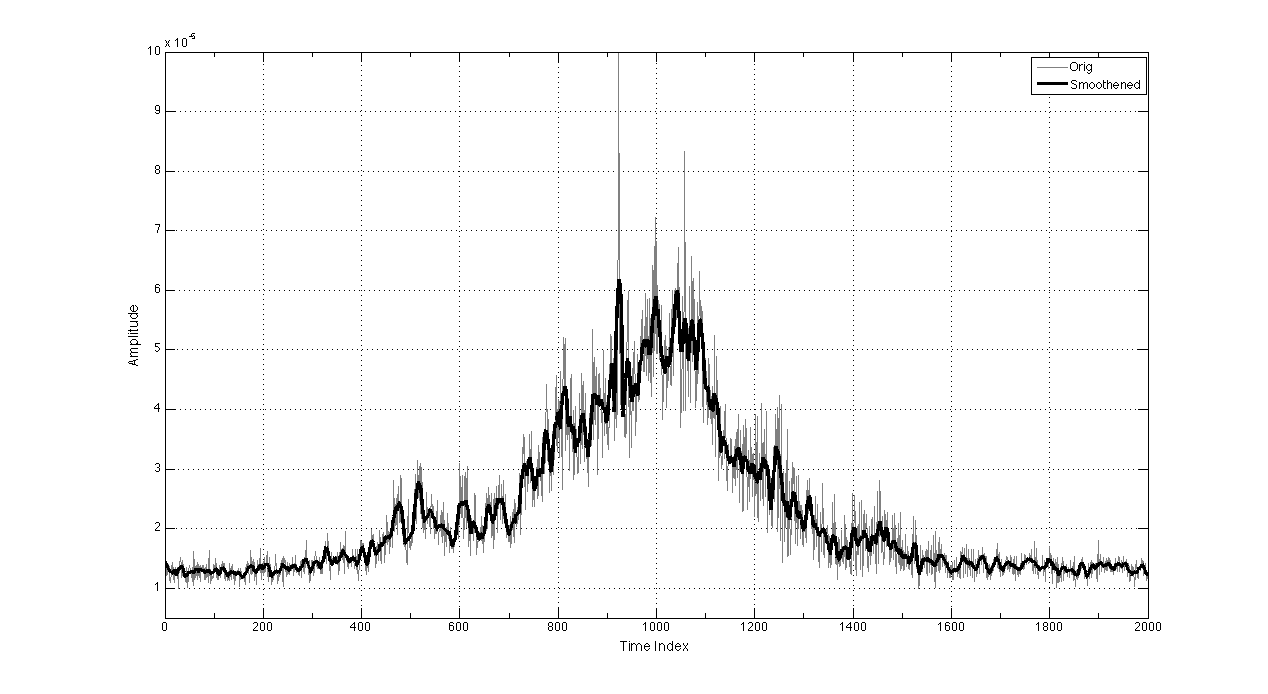
\includegraphics[height=8.4cm]{../images/smoothened.png}
\caption{Effect of the smoothing filter on fluctuating Residual Parameter.}
\end{figure}

\section{Multi-pass Analysis}

\begin{table}
\begin{center}
\begin{tabular}{ | c | c | c | c | }
    \hline
       Tone Frequency & Samples per cycle & Min Window Length & Max Window Length \\ \hline \hline
       40Hz & 1102.5 &  1024 & 8192 \\
       16kHz & 2.75 & 2 & 16 \\ \hline
  \end{tabular}
  \caption{Samples per sinusoidal cycle, and minimum and maximum window length (in the powers of 2) assuming a sampling frequency of 44.1kHz.}
\label{tab:multiPassParam}
   \end{center}
  \end{table}

In a STFT analysis, the choice of the analysis window length is critical. Too short a window and it might not be able to capture enough samples of a low frequency tone to be able to detect it. Too long a window and the high frequency component may have gradually changed within that duration thus making that change undetectable to the STFT analysis. Thus the window length always has to be in the range of $\frac{1}{2}$ to 4 multiples of the length of a sinusoid of any frequency needing to be tracked. Since audio signals are being considered, the frequency range of interest for human perception of tonal information is from 20Hz to about 15-16kHz. This range can be truncated for natural sounds that mostly lie within 40Hz to 16kHz. Table \ref{tab:multiPassParam} shows the minimum and maximum window lengths for a 40Hz tone and a 16kHz tone to be detected correctly.

Hence, no single window length can be used to capture the data in the entire frequency range accurately. This can be overcome in a few ways. Firstly, using a non-sinusoidal function as a basis of the transform instead of a Fourier transform can help to be able to capture much larger frequency range with a single window length. Wavelet based transforms \cite{ref:waveletTransform} are a good example of this method. However, a wavelet based transform deviates from the fundamental aspect of the SMS technique, making the separation of the tonal component complicated and non-intuitive. This method, although valid, was not implemented for this project; instead a simpler multi-pass method was used to capture the data.

\subsection{Frequency Bands and Filtering}

\begin{table}
\begin{center}

\begin{tabular}{ | c | c | c | c | c |}
    \hline
       Window Length & Hop Length & Padded Window Length & Min Frequency & Max Frequency \\ \hline\hline
       128 & 32 & 512 & 344.53 Hz& 2756.2 Hz\\
        512 & 128 & 2048 & 86.13 Hz& 689.06 Hz\\
        2048 & 512 & 32768 & 21.53 Hz & 172.27 Hz\\
        32768 & 2048 & 131072 & 5.38 Hz & 43.06 Hz \\ \hline
  \end{tabular}
  \caption{Window length, the associated Hop Length, Padded Window Length and corresponding calculated minimum and maximum trackable frequencies assuming a sampling frequency of 44.1kHz.}
      \label{tab:multiPassSpecs}
   \end{center}
  \end{table}

To allow the capture of tonal components at all frequencies multiple passes for STFT analysis can be done. For each pass the waveform is analyzed with windows of different lengths, thus making sure that all the frequency components get analyzed with a window that can detect them. Since the window length is changed, the length of the zero padding as well as the Hop length has to change to keep the other parameter compatible. Table \ref{tab:multiPassSpecs} shows the values which might be used for a 3-pass analysis, and the calculated minimum and maximum frequencies that can be tracked based on the $\frac{1}{2}-4$ wavelength assumption. Keeping to the benefits of using lengths with powers of 2, the various window lengths are also chosen in multiples of 4. This is known as a pyramid STFT analysis. Figure \ref{fig:multistftdiagram} shows an illustration of such a multi-pass STFT analysis.

\begin{figure}[ht]
\begin{center}
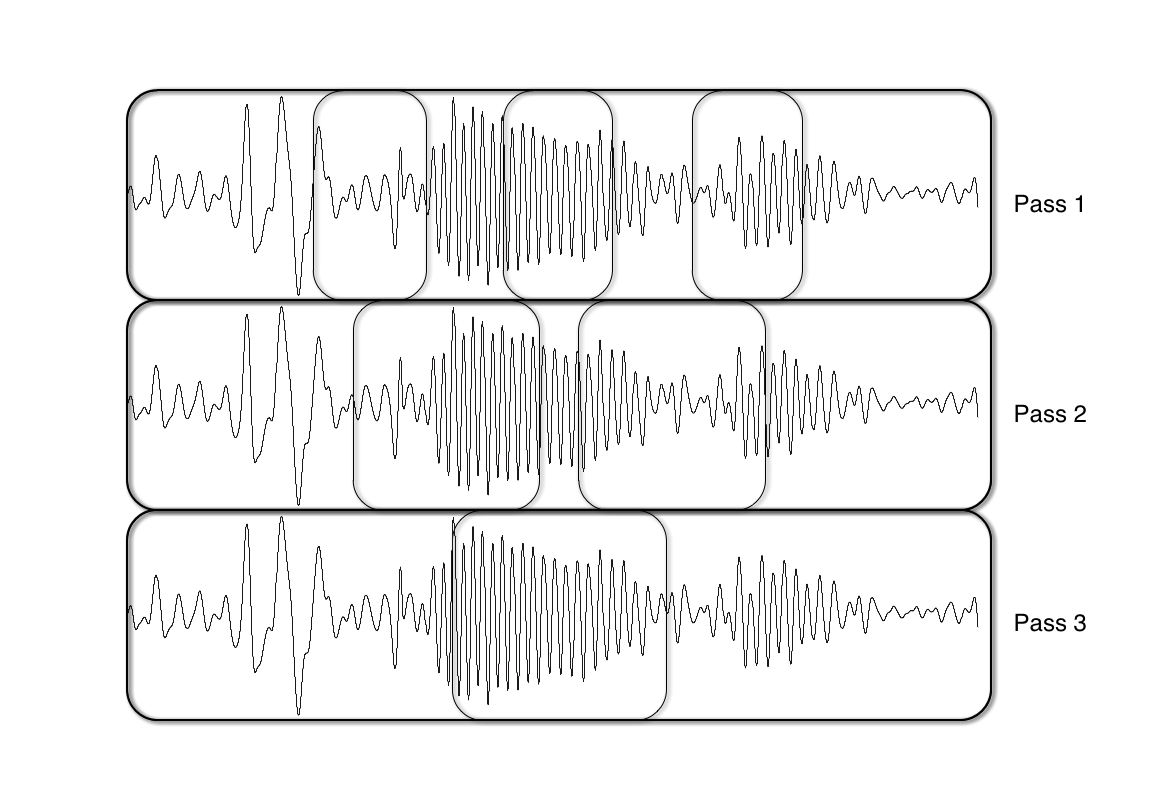
\includegraphics[width=15cm]{../images/MultiPassSTFTDiagram}
\caption{Diagram of a Multi Pass STFT analysis scheme using a sliding windows of various sizes.}
\label{fig:multistftdiagram}
\end{center}
\end{figure}

As a result of multiple passes, a set of peak trajectories are generated for each pass, with different time index lengths between each. However, to force this separation, frequency based filtering has to be done for the peak detection. This ensures that peaks which might be found during the STFT analysis will not be tracked if they do not lie within the band of the frequency which corresponds to the hop length used for the STFT analysis. Thus, assigning a frequency band for each pass, only peaks within the band are considered in the corresponding pass for peak tracking.

Similar filtering is also done for residual calculation. The peak trajectories of each pass are synthesized separately, and used to calculate the separate residuals for each pass. The spectrum of the original sound has to be filtered using the same filters as used in the peak tracking before subtracting the synthesized peak trajectories. This also helps to ensure that the appropriate window length is used for calculating the residual magnitudes, so that the information relevant only to the corresponding frequencies is captured in that residue. During  residual parametrization only the frequencies relevant to the window length are parametrized using filters based on the frequency-bands corresponding to the window length.

For synthesis, since both the peak trajectories and residual parameters have been frequency filtered for each pass, they can be individually synthesized using the STFT parameter for the corresponding pass and finally just summed to generate the final signal.

After tuning for the source data, the values for hop length and corresponding frequency limits shown in table \ref{tab:multiPassFinal} were used.

\begin{table}[ht]
\begin{center}
\begin{tabular}{ | c | c | c | c | c |}
    \hline
       Window Length & Hop Length & Padded Window Length & Min Frequency & Max Frequency \\ \hline\hline
       128 & 32 & 512 & 10000 Hz & 22050 Hz\\
        512 & 128 & 2048 & 4000 Hz & 10000 Hz\\
        2048 & 512 & 32768 & 180 Hz & 4000 Hz\\
        32768 & 2048 & 131072 & 40 Hz & 180 Hz\\ \hline
  \end{tabular}
  \caption{Window length, the associated Hop and Padded Window Length and the Filter Band Limits used in the Multi-Pass Analysis.}
    \label{tab:multiPassFinal}
   \end{center}
  \end{table}

While this method improves the accuracy of the tonal component detection greatly, it adds a significant computational overhead. And especially with very small window lengths, many more frames are generated causing the time taken for the analysis to increase greatly. Hence a balance has to be achieved between computational effort and accuracy of the modeling. A higher number of passes can yield a more accurate model, but also add more computation overhead. However, since most of the computational effort is used for the analysis stage, the synthesis stage can be optimized to run quicker and possibly run in real time for a demonstrator tool.

\subsection{Pass based Guide Limit Assignment}

An attempt to improve the efficiency of the analysis stage was made considering the time taken for peak tracking. At higher frequencies with a greater number of frames, peak tracking takes a significant amount of time. However, most of the tonal energy is in the lower frequencies and most of the trajectories in the short window length pass have too little energy to be considered in the synthesis.

Thus to avoid redundant analysis for tones in the higher frequency ranges, a variable number of guide limit was assigned to each pass, which segregate based on frequency. The pass with large window length, where most of the tonal energy was located was assigned greater number of frequency guides to begin with, while the pass targeting the higher frequencies was assigned fewer guides initially. This reduced the time as well as memory footprint of analysis significantly.

These variable numbers of guide limits is again a parameter that needs to be tuned for the various source sounds. Table \ref{tab:multiPassGuideRatio} shows the values used for the model of the road vehicles and worked well for these types of sounds.

\begin{table}[ht]
\begin{center}
\begin{tabular}{ | c | c | c  | c |}
    \hline
       Window Length & Guide Ratio & Min Frequency & Max Frequency \\ \hline\hline
       128 & 0.05 & 10000 Hz& 22050 Hz\\
        512 & 0.35 & 4000 Hz& 10000 Hz\\
        2048 & 0.4 & 180 Hz& 4000 Hz\\
        32768 & 0.2 & 40 Hz& 180 Hz\\ \hline
  \end{tabular}
  \caption{Window length, the Guide ratio and the Filter Band Limits used in the Multi-Pass Analysis.}
      \label{tab:multiPassGuideRatio}
   \end{center}
  \end{table}

\section{Energy Scaling}
\label{sec:energyscaling}
When the final synthesis of both the tonal and noise components is complete, the two time domain audio signals can be combined by simple addition. However, during the process of analysis, modeling and synthesis, some amount of the total energy might be lost in the simplifications done. While this should not generally matter in the perception of the sound, since the SMS technique is designed to produce perceptibly similar audio, it can affect in a couple of specific instances.

While small changes in overall energy level might not be perceptible, the comparison between the levels of the tonal and the noisy components can be perceived. Such a difference is possible as very different type of algorithms and models are used for the two components and hence energy can be lost in different ways in each of the models. However a mismatch ratio or energy between the two components can be perceived making the final sound noisy or tonal.

Furthermore, the total energy content of the final synthesized signal in comparison to the original signal is important since they too are to be compared. When listened to one after each other, small variations in total energy level are audible as loudness differences in the sounds.

Hence to ensure that lost energy is compensated in an accurate way, energy based amplitude scaling was implemented in various parts of the synthesis section. Such an amplitude scaling method ensures that the total energy of the synthesized section of the sound is equal to the total energy of the corresponding section of the original sound by scaling the synthesized sound by an appropriate amount. Equation \ref{eqn:energyScalingS}-ef{eqn:energyScalingE}- illustrates how this can be done :

\begin{eqnarray}
E_{orig} = &\sum_{0}^{N} x^2 \\
\label{eqn:energyScalingS}
E_{resynth} = &\sum_{0}^{N} x_{resynth}^2 \\
x_{scaled} = &x_{resynth}\times \sqrt{\frac{E_{orig}}{E_{resynth}}}
\label{eqn:energyScalingE}
\end{eqnarray}

Here, $x$ is the original signal, and the $E_{orig}$ is the calculated energy term over the entire signal. $x_{resynth}$ is the synthesized signal and finally $x_{scaled}$ is the scaled version of the synthesized signal.

This ensures that, when combined, the original and re-synthesized sounds are similar in perceived amplitude as well as in the combination of tonal and noisy components.

This scaling was used in a few parts of the synthesis including the synthesis of individual Residual hops; during the combination of synthesized noise and tonal signals; and finally overall on the final synthesized signal to make sure that the energy of the original and synthesized is the same.

\section{Parameter Control}

With the various operations in the SMS method requiring constants which change the way the analysis or the synthesis is done, the method requires a number of parameters. These parameters include, window length ,number of critical band sections, noise threshold, $\alpha$ for peak continuation, guide ratios, sleep interpolation width, peak energy filter minimum value, and the Savitzky�Golay filter parameters.

\begin{table}[ht]
\label{tab:masterParams}
\begin{center}
\begin{tabular}{ | l | l | l |}
    \hline
      Section & Parameter Name & Value \\ \hline \hline
      Multi-pass STFT Analysis & Window Length 1 & 128 \\
      Multi-pass STFT Analysis & Window Length 2 & 512 \\
      Multi-pass STFT Analysis & Window Length 3 & 2048 \\
      Multi-pass STFT Analysis & Window Length 4 & 8152 \\
      Multi-pass STFT Analysis & Filter Band Limits 1 &  10kHz-22kHz \\
      Multi-pass STFT Analysis & Filter Band Limits 2 &  4kHz-10kHz\\
      Multi-pass STFT Analysis & Filter Band Limits 3 &  180Hz-4kHz\\
      Multi-pass STFT Analysis & Filter Band Limits 4 &  40Hz-180Hz\\
      Multi-pass STFT Analysis & Hop Overlap Factor & 75\% \\
      Multi-pass STFT Analysis & Zero Padding Factor & 4 \\ \hline
      Peak Tracking & Noise Threshold & -65dB \\
      Peak Tracking & Max Peaks per Frame & 20 \\
      Peak Tracking & Initial Guide Number & 100 \\
      Peak Tracking & Guide Increment Factor & 0.25 \\
      Peak Tracking & Sections per Critical Band & 25 \\
      Peak Tracking & Guide Ratio 1 & 0.2 \\
      Peak Tracking & Guide Ratio 2 & 0.4 \\
      Peak Tracking & Guide Ratio 3 & 0.35 \\
      Peak Tracking & Guide Ratio 4 & 0.05 \\
      Peak Tracking & $\alpha$ & 0.2 \\
      Peak Tracking & Peak Energy Filter Minimum Value & 0.002 \\
      Peak Tracking & Sleep Interpolation Width & 0.5s  \\ \hline
      Residual Parameterization & Savitzky-Golay Pole Order & 2 \\
      Residual Parameterization & Savitzky-Golay Filter Order & 19 \\ \hline
  \end{tabular}
  \caption{Various parameters used in the Multi-Pass Analysis.}
  \end{center}
\end{table}

The control of these parameters and the interaction of their effect with one another, make a complex set of combinations that can be used for this Spectral Modeling technique. While there are definitely ways to automate the detection and calculation of optimized values of many of the parameters, most require pre-analysis of the sound and can get computationally expensive.

The current manual tuning method for the parameters is only able to tune the SMS for a specific type of sound. To be able to extend the method to various types of traffic sounds or even other source data from road vehicles, the parameters have to be re-tuned manually. Table \ref{tab:masterParams} gives a list of the parameter values generated after tuning the SMS system for the source data used here.

\begin{table}
\label{tab:sms_params}
\begin{center}
\begin{tabular}{| l | l | l |}
\hline
Pass Number & Parameter Name & Parameter Value\\
\hline \hline
Pass 1 & Window Length & 512 \\
Pass 1 & FFT Length & 2048\\
Pass 1 & Hop Length & 128\\
Pass 1 & Lower Frequency Limit & 4000 Hz\\
Pass 1 & Upper Frequency Limit & 22050 Hz\\
Pass 1 & Guide Ratio & 0.2\\
\hline
Pass 2 & Window Length & 2048\\
Pass 2 & FFT Length & 8129\\
Pass 2 & Hop Length & 512\\
Pass 2 & Lower Frequency Limit & 180 Hz\\
Pass 2 & Upper Frequency Limit & 4000 Hz\\
Pass 2 & Guide Ratio & 0.5\\
\hline
Pass 3 & Window Length & 8192\\
Pass 3 & FFT Length & 32768\\
Pass 3 & Hop Length & 2048\\
Pass 3 & Lower Frequency Limit & 20 Hz\\
Pass 3 & Upper Frequency Limit & 180 Hz\\
Pass 3 & Guide Ratio  & 0.3\\
\hline
All & Max number of Peaks & 20\\
All & Noise Threshold (dB) & -65dB\\
All & Critical Band Sections & 25\\
All & Guide Limit Increase Factor & 0.25\\
All & Minimum Guide Energy Factor & 0.02\\
All & Peak Trajectory Smoothing Factor, $\alpha$ & 0.2\\
\hline
\end{tabular}
\caption{Parameters used for sounds in the listening test.}
\end{center}
\end{table}

\section{Propagation Transfer Function}
\label{sec:prop_trans_func}

In a common Auralization scenario, the propagation transfer function is calculated between the source and receiver point and the corresponding time domain impulse response is convolved with the source audio to produce a representation of the audio at the receiver�s position.

However, with the SMS model, another approach opens up as all the information in the model is saved in the frequency domain. The transfer function, which is a scaling for each frequency can be directly applied to the model parameters. Appropriate frequency trajectories can be scaled down by the value of the propagation transfer function at that frequency, and the noise parameters can also be scaled down an averaged value of the propagation transfer function across the respective frequency band. Furthermore, since the SMS model is based on STFT based analysis, it can be used with time based propagation transfer functions, allowing various transfer functions to be applied to various time instances (or frames) of the sound model. This allows the models to be able to directly synthesize the propagated sound, removing a need to store the propagation transfer function and calculate convolution of the impulse response and synthesized sound, which can be computationally intensive.

Care needs to be taken however though as such a use-case may come with its own set of limitation and introduce additional artifacts into the synthesis.

Combined with the propagation transfer function, an SMS based model may be used to generate real time Auralization vehicle sounds at any specified location taken much less time and also reducing memory and computational cost significantly.

\section{Binaural Listening}

For the LISTEN demonstrator, binaural renderings of the source data are needed at the receiver location based on the source model and the propagation data. While most of the binaural calculations have to do with the propagation transfer function, certain aspects of the binaural signal processing are related to the source model. In heavier vehicles and buses, when the engine is located at a different location compared to the wheels, the binaural transfer function for the engine noise and the tire noise is different. While this distinction also exists in a mono synthesis, the perceptual sensitivity of source location is greater in a binaural listening case, hence, in a binaural case is it critical to be able to separate the engine and tires noise sources, and apply separate transfer functions to them based on the locations.

Using the SMS technique the tonal component can be assumed to be the model of the engine noise and the noise component as the contribution of the tires as a rough approximation. This can enable the use of separate transfer functions to generate a binaural listening sound. However, this separation method and its effects were not studied as a part of this thesis project.

\section{MATLAB Implementation}

The entire SMS Analysis/Synthesis system was implemented in MATLAB mainly because of its ability to generate quick prototypes and also because of built-in support for many signal processing libraries and filters. The MATLAB DSP Toolbox had to be used for certain specific functions, but the rest of the system was coded in using the basic MATLAB functionality.

The MATLAB implementation allowed the visualization data, like spectrograms, magnitude spectrums and other parameters, being captured during the analysis as well as rapid testing of effects of parameter sets on the analysis and synthesis. The ability to play back the auralized model in MATLAB, helped to fix many of the issues faced in the modeling of the vehicle noise data. MATLAB scripts were also used in automating the generation of a large number of files which were used as the test data for listening tests.